\subsection{Vulnerabilities in OAuth clients}
When implementing OAuth-based authentication systems, a developer can choose to rely on external authorization servers, greatly simplifying the authentication logic they need to implement on their own.
When relying on external authorization servers, a developer is limited to studying the available providers and choosing ones that are suitable and secure.
This in turn allows developers to focus on implementing a secure client.
The most common client vulnerabilities are related to poor CSRF protections due to misuse of the \textit{state} parameter, poor tracking of user intent and incorrect token storage in the client.

\subsubsection{Invalid state handling}
\label{sec:vulnerabilities-state}
When used correctly, the state parameter provides protection against CSRF attacks \citep{almgren_more_2015}, with the OAuth 2.0 specification stating that the state parameters should be used for all authorization requests.
However, a 2016 study by Yang et al. found that 61\% of studied applications did not use the state parameter, while 55\% of applications that use state mishandled it in some way \citep{yang_model-based_2016}.
A study carried out by Almgren et al. (2015) was less pessimistic, but still found that 25\% of the Alexa Top 10 000 websites did not implement standard CSRF protections, such as correctly utilizing state \citep{almgren_more_2015}.

The OAuth authorization flows utilize redirects to provide access tokens and authorization codes to clients.
If the state parameter is not used by the OAuth client, clients have no way to verify how an authorization flow was initiated.
As such, if the state parameter is missing, many types of CSRF attacks become easier to execute for attackers.
The simplest form of CSRF attack that can be performed on clients that do not use the state value is the login CSRF attack.
In the login CSRF attack, a victim is tricked to authenticate to a legitimate site using the legitimate authorization server, but signing in the victim as the attacker.
This can lead to the victim performing operations as the attacker, and if the victim stores any information while they are logged in, such as payment information, the attacker will gain access to them.

Missing state validation can also be used to attack the federation process of an OAuth system that is used to sign in users \citep{chow_security_2014}.
The attack targets the account creation process, causing the victim's account on a relying site to bind to an account at the provider that is controlled by the attacker.
While the attack is similar to the login CSRF attack, it provides more persistent access to attackers, and has an increased probability of leaking the victim's personal information, as such information is typically provided when creating an account.

While state is used by many clients, it is not very useful if it is not implemented correctly.
Similar attacks can often be performed on clients mishandling the state parameter as on those that do not consider the parameter at all.
The state parameter should be random and difficult to guess, should ideally be single-use and should under no circumstances be shared between sessions or users.
Yang et al. (2016) identified a number of common mistakes in state validation \citep{yang_model-based_2016}:
\begin{itemize}
    \item \textbf{Lack of state validation} \\ 
    The state parameter is used but its value is never actually validated by the client
    \item \textbf{Lenient state validation} \\
    Some clients only validate the state parameter if it is provided. However, they do accept requests that are missing the state parameter.
    \item \textbf{State not bound to user} \\
    The client assumes that all state parameters that it has generated are valid but does not check which user the state parameter belongs to.
    This allows an attacker to perform a CSRF attack by substituting the victim's state with their own.
    \item \textbf{State not single use} \\
    If the state parameter is not single use, an attacker can use a previous parameter in a replay attack.
    The parameter could be obtained by eavesdropping or some other form of leaking.
    The risk for leaking the state parameter is especially high if TLS is not used. Some common characteristics of state reuse are keeping the same state value until the user tries to log in again, keeping the same state value as long as the user uses the same browser, or using a constant state value across all sessions and users.
\end{itemize}

%\subsubsection{Session integrity attack}


%\subsubsection{Poorly configured client authorization}


\subsubsection{IdP mix-up attack}
\label{sec:vulnerabilities-idp}

If the OAuth client fails to keep track of the authorization server that the user has chosen, an IdP mix-up attack could be performed by a network attacker \citep{fett_comprehensive_2016}.
In the IdP mix-up attack, a victim's authorization code or access token is sent to an authorization server controlled by an attacker.
To perform the attack, the OAuth client must allow multiple different authorization servers, and one of the allowed servers must be malicious.
In practice, this could occur if one authorization was compromised by attackers, providing them further access.
An attacker must also be able to modify requests sent to the OAuth client, which could be accomplished by an active network attacker.

The IdP mix-up attack in an authorization code flow is described in figure \ref{idp_mix_up}.
The request initiating authorization (request 1) is modified by an attacker, changing the chosen authorization server from the honest authorization server to a malicious server controlled by the attacker.
The client stores the choice of authorization server locally, and redirects the user agent to the malicious authorization server (requests 2 and 3).
The malicious server redirects the user agent to the honest authorization server, making it very difficult for the victim to notice anything out of the ordinary (request 4).
The end user authenticates normally to the honest authorization server, and the authorization server sends a response containing an authorization code to the OAuth callback route of the client (request 5).
As the client believes that the malicious authorization server should be used, it sends the authorization code to the malicious authorization server when it attempts to request an access token (request 6).
The malicious authorization server now has the victim's authorization code, and can request an access token (requests 7 and 8).
Having gained access to the access token, the attacker can now impersonate the victim or gain access to protected resources belonging to the victim \citep{tonetta_security_2017}.


\begin{figure}[b]
	\centering
    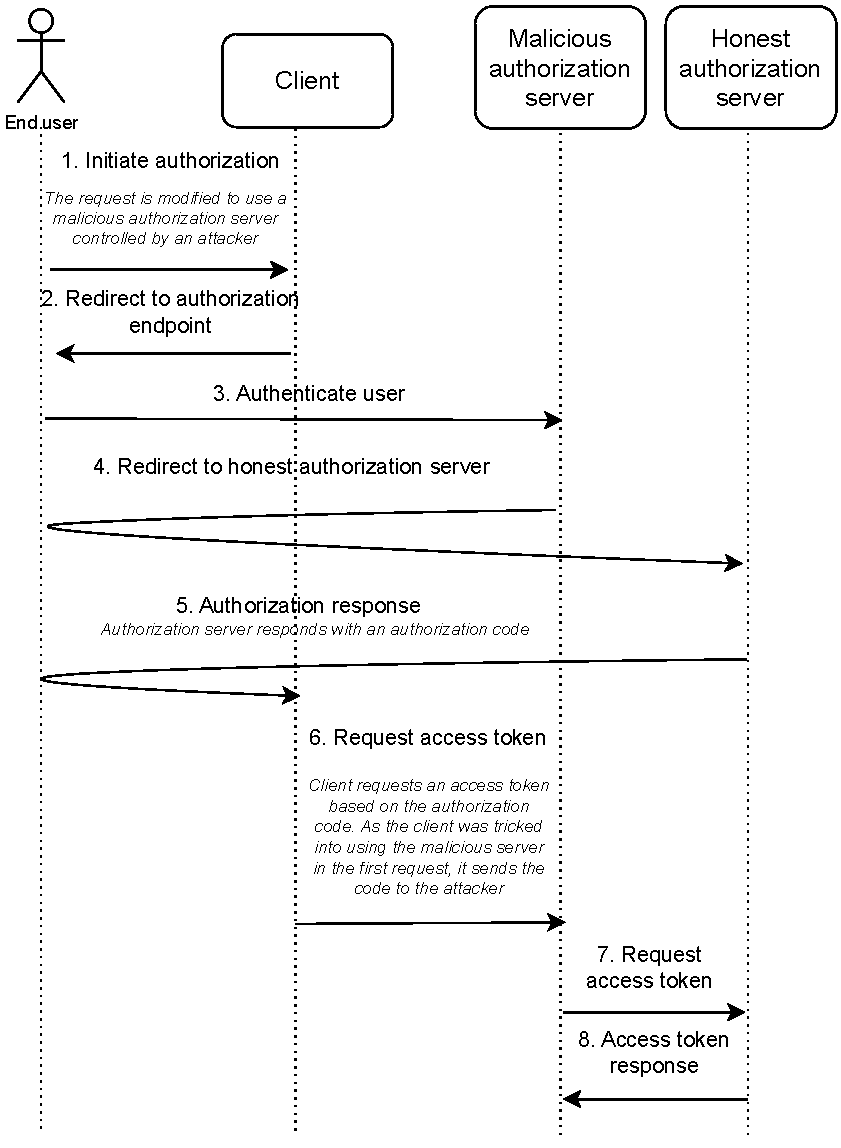
\includegraphics[height=185mm]{assets/idp_mix_up.drawio.pdf}
	\caption{IdP mix-up attack in an authorization code flow}
	\label{idp_mix_up}
\end{figure}

\subsubsection{Vulnerabilities in token storage}
When storing data in web clients, the user will be able to access the data, no matter how much a developer attempts to secure it.
Client-side storage such as cookies or local storage are also vulnerable to XSS attacks.
As such, if the goal is to maximize security, public clients should completely avoid persistent local token storage.

Even if persistent local storage is avoided, sensitive codes and tokens will have to be temporarily stored in JavaScript. 
Developers should consider how this temporary storage is implemented.
One possible hardening option is using JavaScript closures.
When using closures, the variables inside the closure can only be accessed by code inside the definition area of the closure, significantly reducing the chance that a XSS attack would succeed in gaining access to client secrets \citep{taly_automated_2011}.
Browsers also allow running code in web workers, which act as a separate thread.
In addition to allowing concurrent programming, web workers allow executing JavaScript code in an isolated sandbox.
Similarly to closures, this greatly reduces the risk of credentials leaking in case of an XSS attack, as the malicious code would have to be executed in the web worker containing the secret to be able to access it \citep{chinprutthiwong_security_2020}.

While persistent token storage has security issues, the added benefits provided by users being able to stay signed in across multiple sessions and browser restarts can outweigh the costs.
When persisting tokens, developers are limited to using the web storage API and storing session data in cookies.
Data stored using the web storage API and as cookies are limited to a specific domain, making it impossible for malicious sites to directly access the sensitive data.
Both methods are however vulnerable to XSS attacks, as they can be accessed using JavaScript.
When using cookies, XSS attacks can be mitigated by setting the \textit{HttpOnly} flag.
When the flag is set, the cookie can no longer be accessed by arbitrary JavaScript, with the cookie being included in requests to a specific domain.
The web storage API does not provide any protections similar to \textit{HttpOnly} cookies, and as such it should be avoided when storing any sensitive information.
As the cookie value is included in every request, this leaves additional room for potential CSRF attacks, making other types of CSRF protections, such as correctly utilizing the \textit{state} parameter even more critical.